\documentclass[../main.tex]{subfiles}
\graphicspath{{\subfix{../figures/}}}
\begin{document}
The Hermiticity of the Hamiltonian in quantum mechanics is thought of being a necessity for physical behavior of a quantum system. However, in recent decades, the field of non-Hermitian quantum physics has shown major progress, both theoretically and experimentally. Systems of an "open nature", i.e systems being connected to an environment, in nuclear, atomic and optical physics have been accurately described by non-Hermitian Hamiltonians~\cite{nonHermrev}. One of the main properties of non-Hermitian operators is the possibility of exceptional points (EPs). These correspond to points in parameter space where two or more eigenvalues and their corresponding eigenvectors of the operator simultaneously coalesce. Exceptional points have been proposed to have several useful technical applications, and along with the optical microring experiments in 2017, exceptional point sensors successfully increased the sensitivity of current and nano-particle detection~\cite{microring1, microring2}.

Another operator in quantum mechanics which more recently has been studied for its native non-Hermiticity is the Liouvillian superoperator~\cite{recentliou, thermal, steering}. The Liouvillian and its corresponding quantum master equation describe the dynamics in open quantum systems, where the system is coupled to a larger environment. Due to dissipation to the environment in such systems, the Liouvillian is not necessarily Hermitian, which again brings the possibility of exceptional points. EPs in Liouvillian physics affect the dynamics of the density operator, and therefore the evolution of all relevant observables in the system. Recently, exceptional points in the Liouvillian have been theoretically studied in quantum thermal machines, where critical decay towards the steady state was found at the EP~\cite{thermal}; and in quantum control, where an EP corresponded to optimal steering toward a target quantum state~\cite{steering}. 

Another application of interest for quantum master equations and Liouvillian physics is electron transport in systems of quantum dots connected to metallic leads~\cite{qdottrans}. A quantum dot is a fabricated semiconductor structure containing a small number of electrons and is typically in the order of 100s nanometres in size (?). The size of the dot needs to be small in comparison with the thermal wavelength of the electrons, which is why experiments are generally realized at temperatures close to absolute zero~\cite{transport}. One method of creating this isolation of electrons is to apply voltages via nanoscale electrodes, called gates, which depletes the number of electrons in a small region, see figure~\ref{fig:sem}. If the voltages are tuned successfully, the quantum dot can be tunnel coupled to the two surrounding conducting regions of the semiconductor, known as the source and drain. The electrons can then tunnel from the source into the dot and then exiting it by tunneling into the drain, producing a current through the system~\cite{qdotmarcus}. This process is schematically presented in figure~\ref{fig:qdotscheme}.

\begin{figure}[H]
    \centering
    \begin{minipage}[t]{0.45\textwidth}
        \centering
        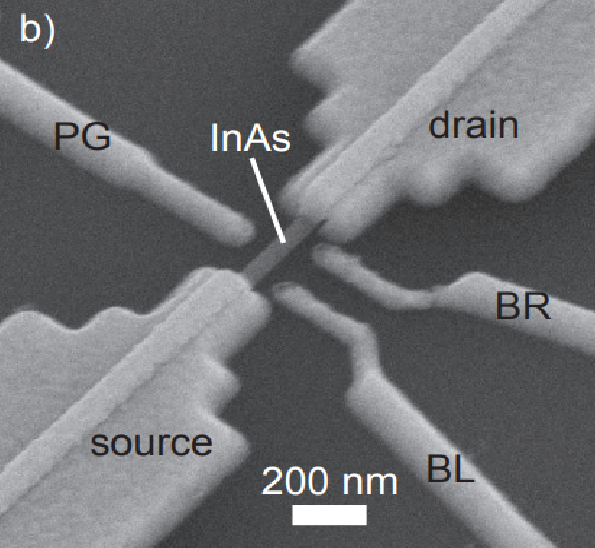
\includegraphics[width=0.8\textwidth]{figures/qdotsem.png}
        \caption{A physical implementation of a single quantum dot system. The quantum dot, labeled with InAs, the source and drain, and the gates (BR, BL and PG) are all clearly visible in this figure, captured by a scanning tunneling microscope. The figure is taken from reference~\cite{sven}.}
    \label{fig:sem}
    \end{minipage}\hfill
    \begin{minipage}[t]{0.45\textwidth}
        \centering
        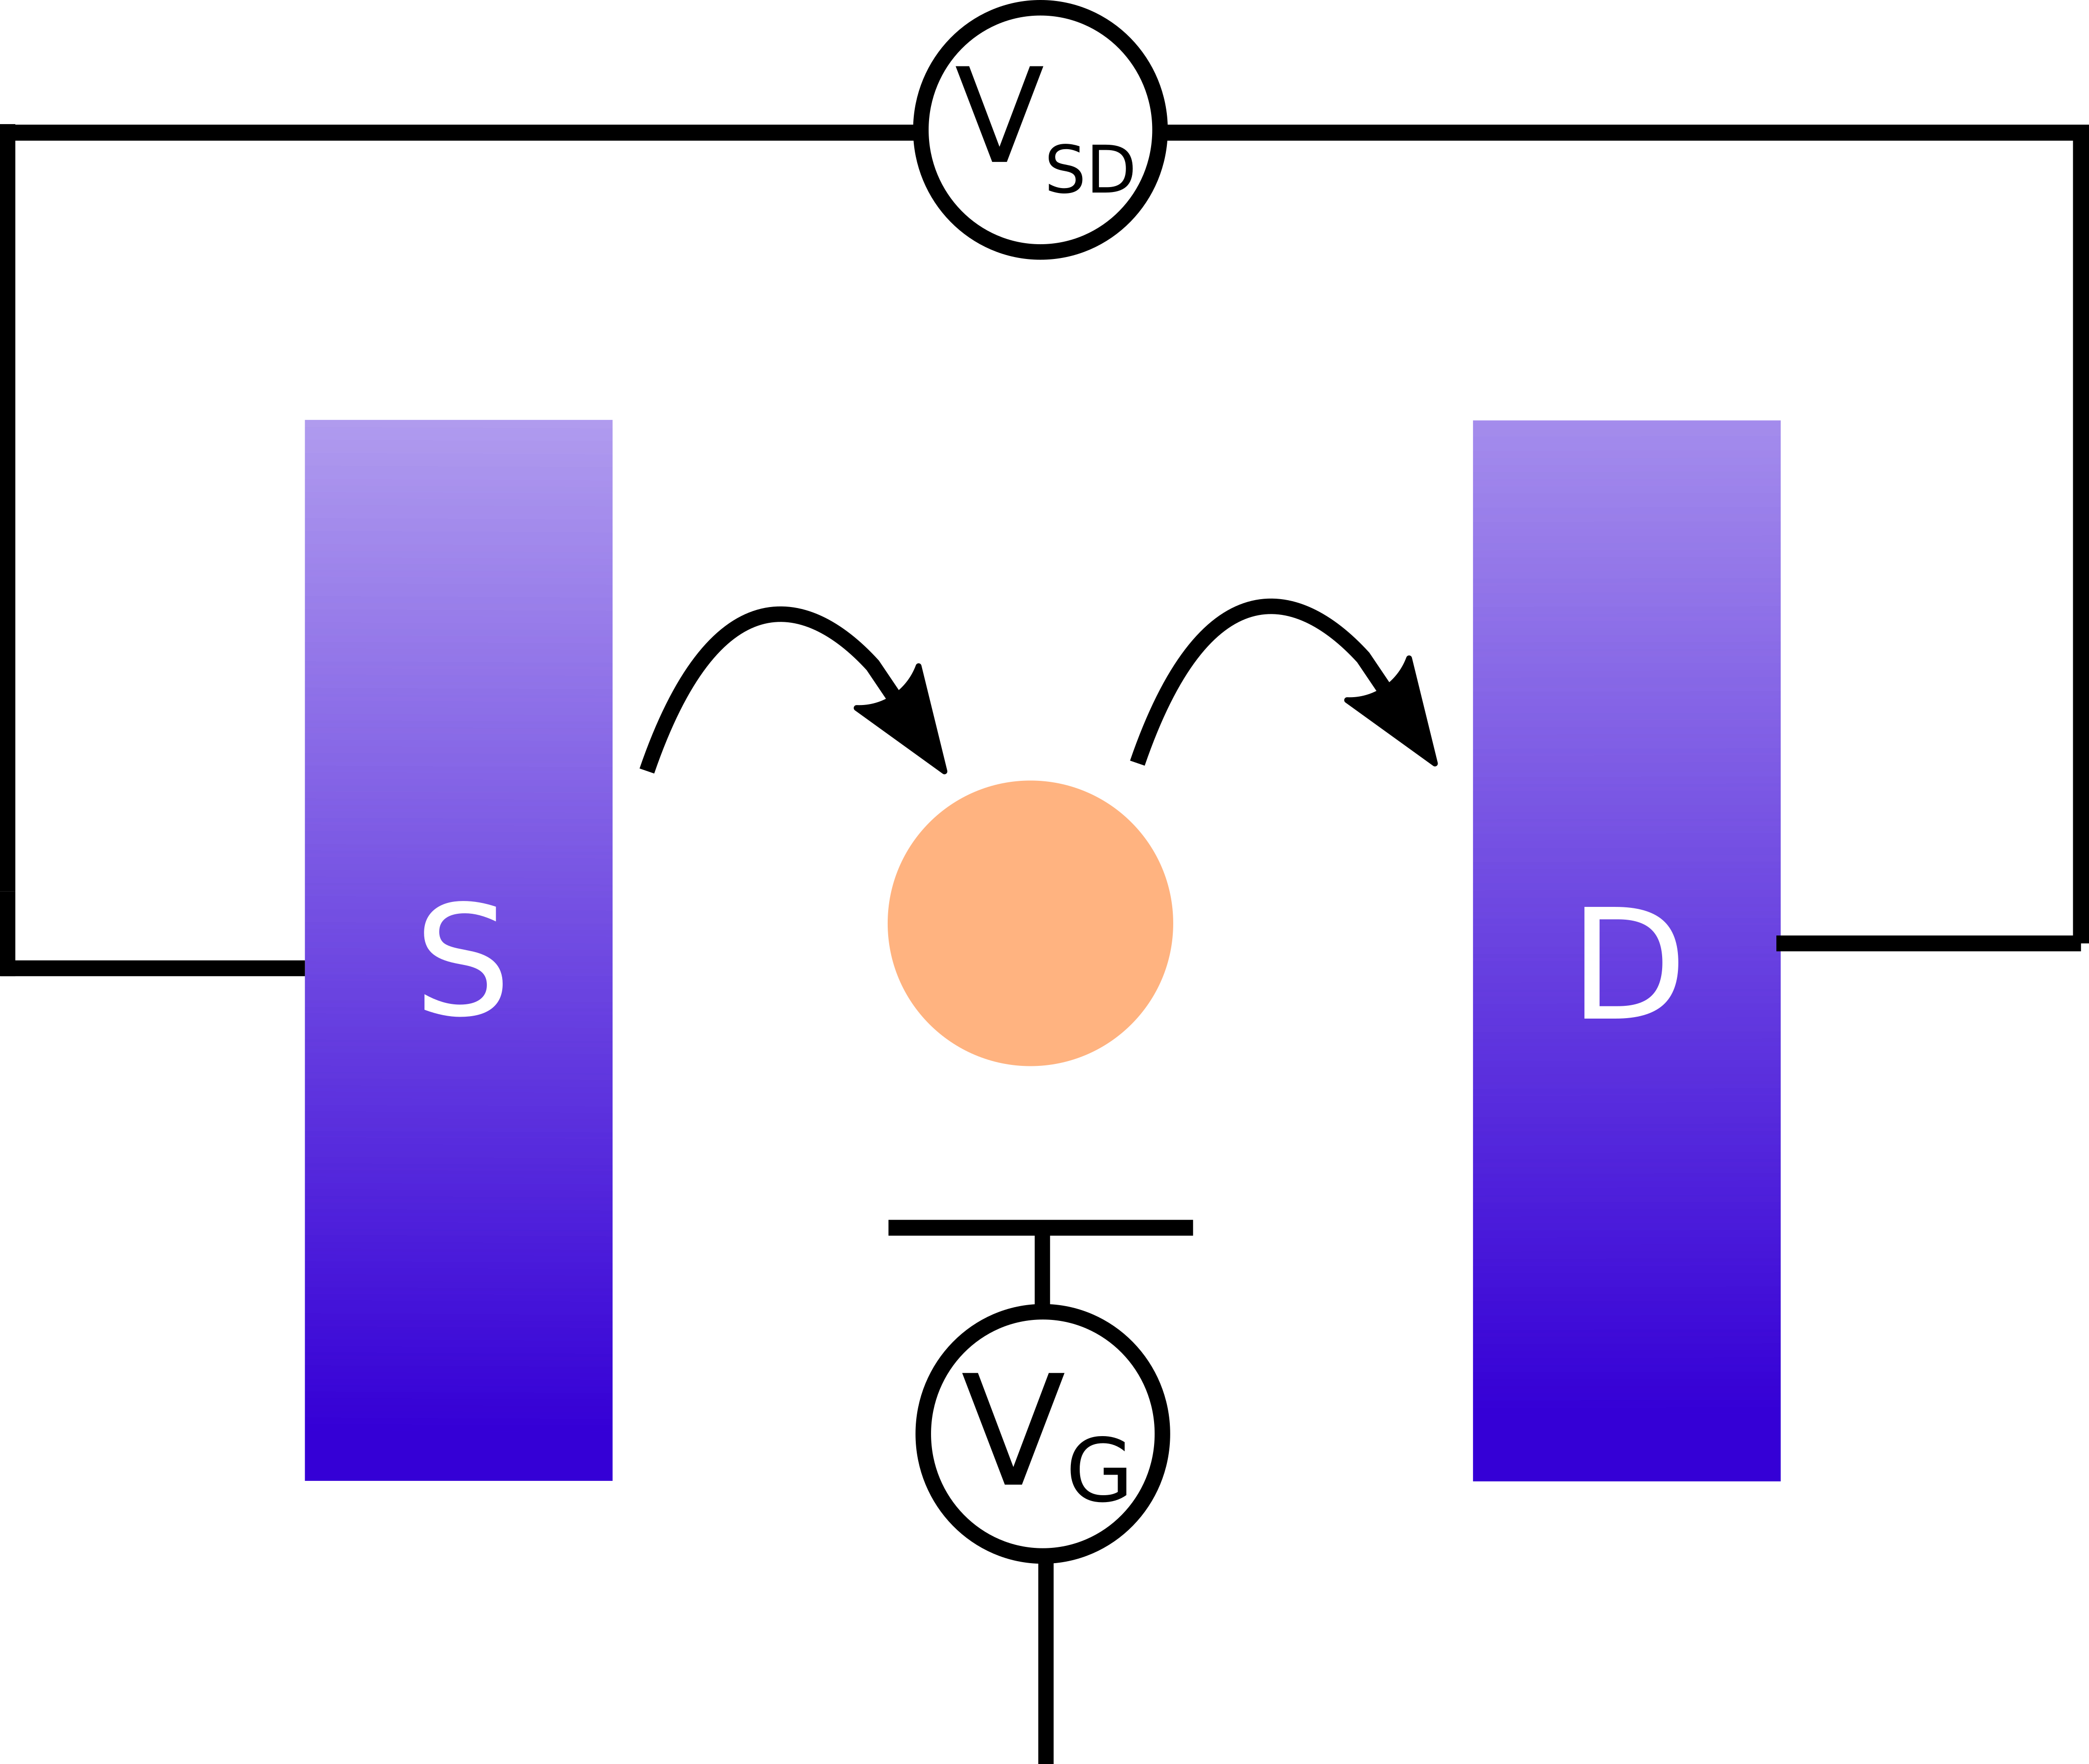
\includegraphics[width=\textwidth]{figures/qdotschematic.png}
        \caption{A schematic figure of a quantum dot system, where the quantum dot is in the center, tunnel coupled to the source (S) and drain (D). The gate voltage $V_\text{G}$ and the source-drain voltage $V_\text{SD}$, are tuned to define the quantum dot.}
    \label{fig:qdotscheme}
    \end{minipage}\hfill
\end{figure}

The system considered in this thesis consists of two quantum dots coupled to two metallic leads, corresponding to the source and drain. The dots are assumed to be coupled in parallel, i.e not directly coupled to each other but only indirectly through the two leads, see figure~\ref{fig:model}. The dynamics of the current through the system can be derived from the microscopic properties of the system, resulting in a quantum master equation and a corresponding Liouvillian. The matrix representation of the Liouvillian will depend on the tunnel coupling strengths, the gate and drain voltages, and the other parameters in figure~\ref{fig:model}. It is in this parameter space in which it is possible to find exceptional points.

\begin{figure}[H]
    \centering
    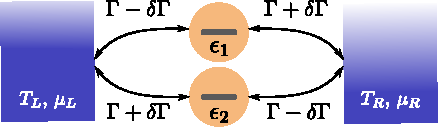
\includegraphics[width=0.8\linewidth]{model.pdf}
    \caption{A model of the system containing two quantum dots (yellow) coupled in parallel to metallic leads (blue).}
    \label{fig:model}
\end{figure}

Go through results and discussion...


\end{document}

